\chapter{Integrating Erratum to Cerberus}

\section{Abstract}
Web applications are constantly evolving to integrate new features and fix reported bugs.
However, even an imperceptible change can sometimes entail significant modifications of the \emph{Document Object Model} (DOM), which is the underlying model used by browsers to render elements of a web application.
In this context, the continuous evolution of web applications makes it extremely challenging to automate test scenarios of a web application in a robust way.
More precisely, the major cause of breakages observed in integration tests are \emph{element locators}, which are identifiers used by automated tests to navigate across a DOM.
When this DOM evolves, these locators tend to break, thus causing the related tests to no longer locate the intended target elements.

So far, established test automation frameworks adopted by the industry, like \cerberus{}, only support CSS or XPath selectors to query web page elements.
Such web locators require to be manually crafted and are often fragile with regards to DOM changes, hence often requiring testers to fix the broken test scenarios in priority. 
While several solutions to this problem have been proposed in the scientific literature, to our knowledge, no locator repair or locator generator has been integrated in open-source test-automation software before.
This paper thus reports on the seamless integration of a more robust web locator in \cerberus{} by leveraging a new locator repair solution, named \erratum{}. While \erratum was originally designed to repair broken locators, this paper demonstrates how it can be extended to deliver an elegant robust locator solution that succeeds to reduce the maintenance cost of automated tests.

\section{Introduction}
The implementation of automated tests on web applications (apps) requires software engineers to locate specific elements in the DOM (\emph{Document Object Model}) of a web page.
To do so, software testers or automation/testing tools often rely on CSS (\emph{Cascading Style Sheets}) or XPath selectors to query the target elements they need to interact with.
Unfortunately, such statically-defined locators tend to break along time and deployments of new versions of a web application.
This often results in the failure of all the associated test scenarios that apply to the modified web pages.

Several existing works focus on repairing tests on GUI applications, but there are surprisingly very few test repair solutions targeting web interfaces~\cite{imtiaz2019systematic}.
These solutions either propose to \emph{i)} generate locators that are robust to changes (so-called \emph{robust locator problem}), or \emph{ii)} repair locators that are broken by the changes applied to the web pages (so-called \emph{locator repair problem}).
Unfortunately, most of the existing solutions in the literature fail to accurately fix a broken locator, thus leaving all the related automation tests as broken~\cite{hammoudi2016record}.

While we already introduced \erratum{},\footnote{\erratum{} stands for "\erratumlong{}"} as an holistic approach to the locator repair problem~\cite{brisset2021erratum}, this paper explores its extension to address the robust locator problem.
More specifically, we report on the integration of \erratum{} in an open-source test automation solution called \cerberus{}~\cite{cerberus-icst20}.\footnote{\url{https://cerberus-testing.com/}}
\cerberus{} is commonly adopted by several companies to write, organize, and run their test campaigns.
In particular, we worked in close collaboration with the web testing team of \laredoute{},\footnote{\url{https://www.laredoute.com/}} a large (846M turnover, $1,700$ employees) french online fashion retailer.

The teams we worked with acknowledged that locator breakage is a painful issue for them that even caused a whole test campaign to be cancelled.
Yet, to the best of our knowledge, none of the locator generator or locator repair solutions existing in the literature have ever been integrated in an open-source testing software.
As a matter of assessment, we observed that the concept of locator repair was unknown to all professional testers we interviewed.


The remainder of this paper is organized as follows.
Section~\ref{sec:related-work} introduces the necessary background on web locators.
% 
Then, Sections~\ref{sec:erratum} and~\ref{sec:cerberus} overview \erratum and \cerberus, respectively, while Section~\ref{sec:integration} reports on the integration of a robust locator solution in \cerberus based on \erratum.
Section~\ref{sec:impact} discusses the preliminary impact of this integration on the software development projects managed by \laredoute.
% 
% Section~\ref{sec:locator} formalizes the locator problem we address in this paper.
% Section~\ref{sec:implementation} introduces our approach, \erratum, which leverages an efficient flexible tree matching solution that we identified.
% Section~\ref{sec:benchmark} describes the locator benchmark we designed and implemented.
% Section~\ref{sec:evaluation} reports on the performance of our approach compared to the state-of-the-art algorithms.
% Section~\ref{sec:threats} discusses the threats to validity of our contribution.
Finally, Section~\ref{sec:perspectives} presents some perspectives for this work, while Section~\ref{sec:conclusion} concludes.

\section{Background}\label{sec:related-work}
\subsection{Web Element Locators}
To detect regressions in web applications, software engineers often rely on automated web-testing solutions to make sure that end-to-end user scenarios keep exhibiting the same behavior along changes applied to the system under test.
Such automated tests usually trigger interactions as sequences of actions applied on selected elements and followed by assertions on the updated state of the web page.
For example, \emph{"click on button $e_1$, and assert that the text block $e_2$ contains the text '{\tt Form sent}'"}.
To build such test scenarios, a software engineer can
\begin{inparaenum}
    \item manually write web test scripts to interact with the application,
    \item use record/replay tools~\cite{burg2013interactive,sen2013jalangi,mickens2010mugshot} to visually record their scenarios, or
    \item adopt low-code test libraries to leverage the description of actions for domain experts.
\end{inparaenum}
In all these cases, the scenario requires to identify the target elements on the page [$e_1$, $e_2$] in a deterministic way, which is usually achieved using XPath, a query language for selecting elements from an XML document.
% 
For example, let us consider the following HTML snippet describing a web form:
\begin{lstlisting}
<form method="post" action="index.php"> 
    <input type="text"   name="username"/> 
    <input type="submit" value="send"/>
</form> 
\end{lstlisting}

The following XPath snippets describe 3 different queries, which all result in selecting the submit button: \lstinline!/form/input[2]!, \lstinline!/form/input[@value="Send"]!, \lstinline!input[@type="submit"]!.
In the literature, such element queries or identifiers are named \emph{locators}~\cite{leotta2014reducing}.

In practice, automated tests are often subject to breakages~\cite{hammoudi2016record}.
While there can be many causes to test breakage, Hammoudi~\emph{et~al.}~\cite{hammoudi2016record} report that $74\,\%$ of web tests break because one of the included locators fails to locate an element in a web page.

\subsection{Web Locator Terminology}
When a locator is defined, manually or automatically, it is written from and for a given web page.
The internal representation of a web page by the browser is a \emph{Document Object Model} (DOM).
In this paper, we adopt the following notations:
\begin{compactitem}
    \item we denote $D$ the original DOM of the web page for which the locator was written and $D'$ an evolution of $D$ on which the locator is expected to work,
    \item we note $e \in D$ an element of the DOM $D$ and $e'\in D'$ the corresponding element in $D'$,
    \item we note $loc_{e, D}$ a locator that identifies $e$ in $D$,
    \item then by construction, evaluating this locator on $D$ returns the original element $e$: $eval(loc_{e, D}, D) = e$,
    \item finally, we assume there is a locator breakage if $eval(loc_{e, D}, D') \neq e'$.
\end{compactitem}

The robustness of a locator can be characterized by its capability to keep selecting the element $e$ on any mutation of $D$.
In the following section, we therefore report on how we integrated \erratum---an effective solution to the locator repair problem---into the \cerberus web testing framework to implement an elegant solution to the robust locator problem, thus addressing a major concern of web testers.

\section{Repairing web locators with \erratum}\label{sec:erratum}
\erratum was developed as a locator repair solution. 
Given a locator $loc_{e, D}$ broken on a new page $D'$, \erratum allows to relocate $e$ on $D'$---\emph{i.e.}, to find $e' \in D'$.
Formally, a locator repair solution, like \erratum, is defined as a function: $(D', loc_{e, D}) \to e'$.

\erratum differs from other locator repair solutions by using an holistic approach: all the elements from $D$ and $D'$ are matched by a efficient tree matching algorithm, and the resulting matching is processed to relocate all elements from $D$ in $D'$~\cite{brisset2021erratum}.

\begin{ex}
Given the Google search page $D$, the send button $e$ is located by the XPath locator $loc_{e,D} = /html/body/div[3]/button$.
Some time later, the page may evolve to $D'$.
Evaluating $loc_{e,D}$ on $D'$ yields no result as the button is now in a wrapped inside a \textsf{form} tag.
In such a situation, \erratum{} can automatically repair the broken locator $loc_{e,D}$ by detecting that the matched element $e \to e'$ is a now child of node \textsc{form}, hence located with $loc_{e',D'} = /html/body/div[3]/form/button$.
\end{ex}

The core of \erratum approach is a tree-matching solution called Similarity Based Flexible Tree Matching (SFTM)~\cite{brisset2020sftm}. 
Given two trees $D$ and $D'$, the SFTM algorithm allows to create a mapping between all elements $e \in D$ and $e' \in D'$.

\erratum then uses this mapping to relocate all locators defined in $D$ in $D'$.

While many tree-matching solutions have been developed, SFTM was specifically designed to accurately match complex web pages with fast response times (below 100ms) and accurately.
To do so, SFTM relies on a distinctive characteristic of DOM trees: the \emph{labels}, which usually contain a lot of information (attributes, attribute values, tags, and inner text).

SFTM thus relies mostly on the labels of the trees and only makes use of topology in a second step, to fine-tune the estimated matchings.
Intuitively, matching two sets of labels is significantly easier than trying to match trees, which is the reason why SFTM achieves such competitive performances.

We walk through the key steps of the SFTM algorithm we integrated in \erratum{} by using HTML snippets reported in Figure~\ref{fig:example_html}.
The figure provides two versions ($D$ and $D'$) of a simplified HTML code sample extracted from the homepage of the search engine \textit{duckduckgo.com}.
In this example, our purpose is to relocate $\text{a}_1 \in D$ with $\text{a}_1' \in D'$.

% \begin{figure}
%   \centering
%   \begin{subfigure}[b]{0.5\linewidth}
%   \centering
%     \begin{lstlisting}[]
%     for i:=maxint to 0 do
%     begin
%     { do nothing }
%     end;
%     \end{lstlisting}
%     \caption{A listing}
%   \end{subfigure}
%   \hfill
%   \begin{subfigure}[b]{0.5\linewidth}
%     \centering
%     \rule{1.5cm}{1.5cm}
%     \caption{A diagram}
%   \end{subfigure}
%   \caption{A listing and a diagram}
% \end{figure}
\begin{figure}
    \centering
    \begin{subfigure}[b]{\linewidth}
        \centering
        \caption{Original document $D$.}
        \begin{lstlisting}[language=html, label={fig:first_version}]
<div class="content-info__item"> /*!\mymk{div_1}!*/
    <div class="item__title">...</div> /*!\mymk{div_2}!*/
    <div class="item__subtitle"> /*!\mymk{div_3}!*/
        ... 
        <a href="/plugins">Plugins</a> /*!\mymk{~a_1~}!*/
    </div>
</div>
        \end{lstlisting}
    \end{subfigure}
    \hfill
    \begin{subfigure}[b]{\linewidth}
        \centering
        \caption{Updated document $D'$ from $D$.}
        \begin{lstlisting}[language=html, label={fig:second_version}]
<div class="items-wrap"> /*!\mymk{div'_4}!*/
    <div class="item"> /*!\mymk{div'_1}!*/
    <div class="item__title">...</div> /*!\mymk{div'_2}!*/
        <div class="item__subtitle"> /*!\mymk{div'_3}!*/
            ... 
            <a href="/extensions">Extensions</a> /*!\mymk{~a'_1~}!*/
        </div>
    </div>
    <div> /*!\mymk{div'_5}!*/  
        ...
        <a href="/newsletter">Newsletter</a> /*!\mymk{~a'_2~}!*/
    </div>
</div>
        \end{lstlisting}
    \end{subfigure}
    \caption{Two versions of an HTML snippet extracted from the homepage of \emph{duckduckgo.com}.}
    \label{fig:example_html}
\end{figure}

Unlike the state-of-the-art matching algorithms, SFTM first tries to match elements in $D'$ whose labels are similar to $D$, before using these matched elements to adjust the similarity of surrounding elements in the tree.
For example, the \emph{similarity scores} of the tuple $(a_1,a'_1)$ links will increase as their direct parents $(div_3,div'_3)$ are matched with confidence.
% 
Figure~\ref{fig:steps_sftm} summarizes the SFTM algorithm's key steps and the remainder of this section provides an overview of its integration in \erratum{} first and then Cerberus.

\paragraph{Step\,1: Node Similarity}\label{sec:node_similarity}
Elements of DOMs $D$ and $D'$ are compared. 
The first step consists in computing an \emph{initial similarity} $s_0 : D \times D' \to [0, 1]$.
For each pair of nodes $(e, e') \in D \times D'$, $s_0(e,e')$ measures how similar the labels of $e$ and $e'$ are.
In HTML pages, the label of a node $e \in D$ that we use is the set of tokens obtained from applying a tokenizer to the HTML code describing $e$. 
This may include the type of the HTML element, its attributes, and eventually the raw content associated to this element---\emph{i.e.}, thus ignoring the content from the child elements.
% After empirically comparing different settings, we noticed that the algorithm performed better (and faster) when ignoring the content of the elements thus only using the tag name and attributes.
% For example, the label of $div_1$ is the following set of tokens $\{\text{div}, \text{class}, \text{content-info__item} \}$
\begin{ex}
The \emph{label} computed for $div_1$ (cf. Figure~\ref{fig:example_html}) includes the following tokens: $\{\texttt{div}, \texttt{class}, \texttt{content-info\_\_item} \}$. %The algorithm ignores the content.
\end{ex}
% For example, the label of $div_1$ is the following set of tokens $\{\text{div}, \text{class}, \text{content-info\_\_item} \}$

To compute $s_0$, SFTM first indexes the labels of each node of $D$.
The idea of this step is to prune the space of possible matches by pre-matching nodes with similar labels.
When indexing, to improve the accuracy of $s_0$, we apply the \emph{Term Frequency-Inverse Document Frequency} (TF-IDF)~\cite{jones1972statistical} formula to take into account how rare each token is.
\begin{ex}
    Following our previous Example~\ref{fig:example_html}, when considering the match $(div_1, div'_1)$:
    \begin{compactenum}
        \item token $\texttt{div}$ will yield very few similarity points, since it is included in the labels of almost all the nodes,
        \item token $\texttt{content-info\_\_item}$ will increase the score significantly, as it only appears once in both documents.
    \end{compactenum}
\end{ex}
% Following our previous example~\ref{fig:example_html}, when considering the match $(div_1, div'_1)$:
% \begin{compactenum}
% \item the token $\text{div}$ that both elements have in common will yield very few similarity points since it appears in the labels of almost all nodes.
% \item The token $\text{content-info\_\_item}$ will increase the score significantly as it only appears once in both documents.
% \end{compactenum}

In general, very common tokens bring very few information to the relevance of a given match, while they cause a significant increase of potential matches to consider.
That is why, in order to reduce the computation times, the algorithm rules out most common tokens.

\paragraph{Step\,2: Similarity Propagation}
The initial similarity $s_0$ only takes into account the labels of nodes.
In this second step, the idea is to enrich the information contained in $s_0$ by leveraging the topology of the trees $D$ and $D'$.
\begin{ex}
    In Example~\ref{fig:example_html}, it is hard to choose the correct match $m_1 = (a_1, a'_1)$ over the incorrect one $m_2 = (a_1, a'_2)$ by only considering labels, since all three elements share the same set of tokens: $\{\texttt{a}, \texttt{href}\}$.
    In the similarity propagation step, we leverage the fact that the parents of $a_1$ and $a'_1$ are similar to increase the similarity between $a_1$ and $a'_1$, thus preferring $m_1$ over $m_2$.
\end{ex}
% In our example~\ref{fig:example_html}, it is hard to choose the correct match $m_1 = (a_1, a'_1)$ over the incorrect one $m_2 = (a_1, a'_2)$ using only labels since all three elements have the same set of tokens in common: $\{\text{a}, \text{href}\}$. In the similarity propagation step, we use the fact that the parents of $a_1$ and $a'_1$ are similar to increase the similarity between $a_1$ and $a'_1$ which allows to successfully choose $m_1$ over $m_2$.
In general, for each considered match $(e, e') \in D \times D'$, the parents of $e$ and $e'$ gets more similarity points if $e$ and $e'$ are similar and inversely, $s(e, e')$ is increased if the parents of $e$ and $e'$ are similar (with regard to $s_0$).
We call $s$ the final similarity produced by this step.

\paragraph{Step\,3: Optimization}
Producing the optimal matching with regards to the computed similarity means selecting the full set of matches such that each element of $D$ is matched with at most one element of $D'$ and the sum of similarity scores of the selected matches is maximum.

In order to approximate the optimal set of matches, SFTM implements the Metropolis algorithm~\cite{metropolis1953equation}.
The idea is to randomly walk through several possible configurations (set of matches) to converge towards the optimal one.

\begin{figure*}[!t]
    \centering
    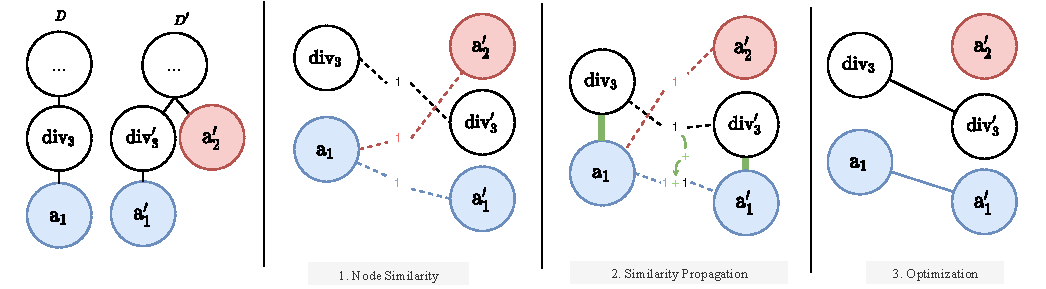
\includegraphics[width=0.8\linewidth]{cerberus/explanations/sftm}
    \caption{Key steps followed by our \emph{Similarity-based Flexible Tree Matching} (SFTM) algorithm.}
    \label{fig:steps_sftm}
\end{figure*}

At the end of the optimization step, the SFTM algorithm yields a full matching $M \subset D \times D' $ comprising matches between nodes of $D$ and $D'$.
These matches can be further analyzed by \erratum{} to locate broken locators and fix them by generating new locators in the target document $D'$.

\section{Building test cases with \cerberus}\label{sec:cerberus}
\cerberus is a low-code open source scalable test automation solution.
It is used by several large companies to create, organize, and run their test suites.
\cerberus contains many features, including parallel test execution, test requirement management, and reporting.
We integrated \erratum in one of the core component of \cerberus: the test case creation.\footnote{\url{https://github.com/cerberustesting/cerberus-source/issues/2252}}

A test case in \cerberus describes a sequence of \textit{actions} to be executed.
Each action has a type and specific arguments that match this type.
Figure~\ref{fig:cerberus} depicts the action editor of \cerberus.
For most action types, the main required argument is the \textit{locator} ("element path" in the screenshot)---\emph{e.g.}, if the action is "click", the locator refers to the element on which \cerberus should click.
The action "form" allows the tester to specify the locator using element properties, like \textit{id}, \textit{class}, \textit{name}, or use more expressive query languages, like CSS or XPath.
Nonetheless, there are mainly two drawbacks to such basic queries:
\begin{compactitem}
    \item defining the robust locator of an element is a tedious and often arbitrary task,
    \item tests tend to quickly break because the underlying locators break.
\end{compactitem}

\begin{figure*}[]
    \centering
    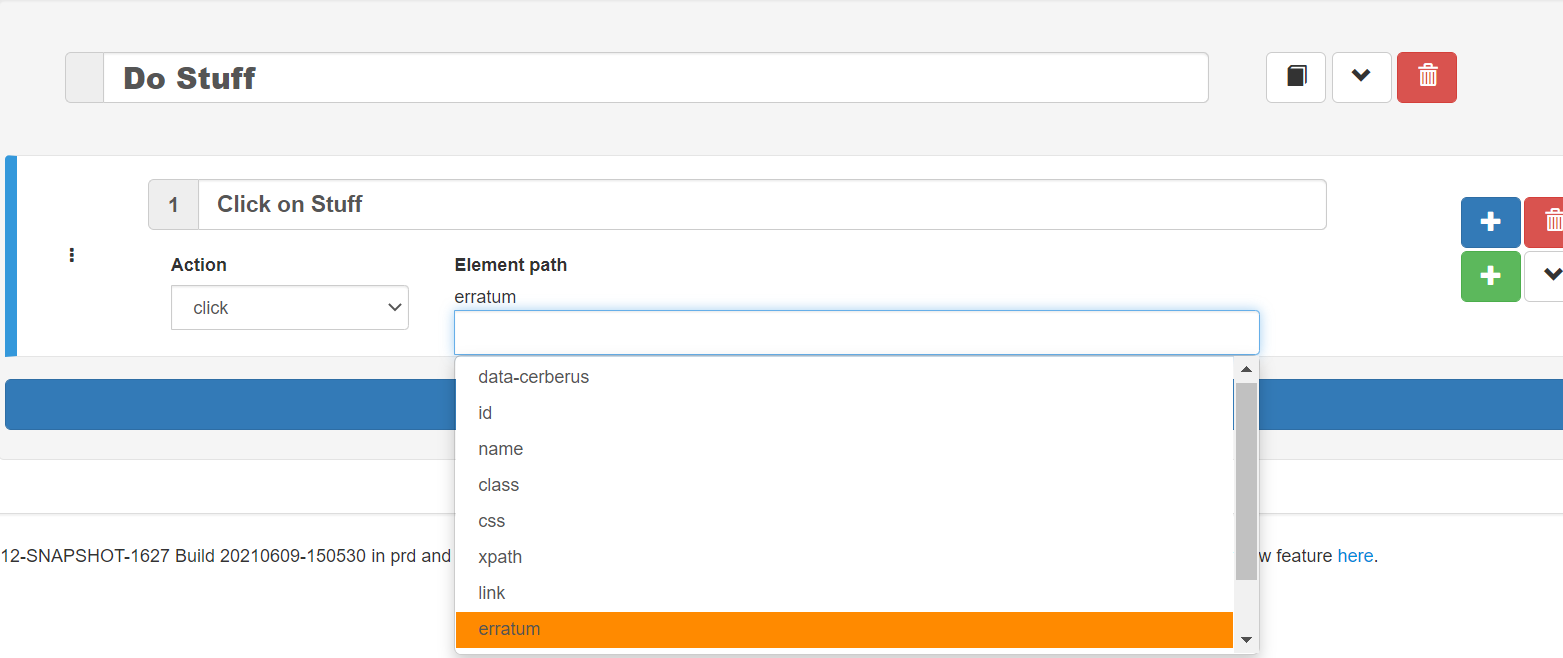
\includegraphics[width=.85\linewidth]{cerberus/explanations/cerberus}
    \caption{A screenshot of the \cerberus web interface to define a test case.}
    \label{fig:cerberus}
\end{figure*}

It appears that these drawbacks are more than a mere inconvenience. 
When first meeting with one of the companies interested in \erratum, we were told that a whole test campaign had to be discarded because the locators included in the considered test cases were constantly breaking during the software development process.

To overcome these problems, \cerberus standardized the use of \textit{data-cerberus} identifiers, which are simple element attributes aimed at uniquely identifying web elements to be used by automated tests.
For example, if developers anticipate that the web testing team needs to interact with a specific application button, they should include such an identifier as follows:
 \begin{lstlisting}
    <button data-cerberus="a_special_button" type="button">Send</button>
\end{lstlisting}

Unfortunately, using such static identifiers entails other challenges, among which:
\begin{compactenum}
    \item it introduces a---probably undesired---tight coupling between the development and testing teams,
    \item if a \texttt{data-cerberus} attribute is missing, the development team should first fix the page under test and then re-deploy the web application, which may take time and several iteration to expose all the required identifiers,
    \item for various reasons, the testing team might not have the possibility to change the source code of the page under test (\emph{e.g.}, proprietary source code), and finally
    \item it forces web developers to anticipate and maintain all these unique identifiers to ensure the absence of identifier collision.
\end{compactenum}

The above observations shared by testing practitioners from \laredoute{} and \cerberus demonstrate that none of the standard locators support a robust execution of their test campaigns.
In the best case, they reported that broken locators causing the failure of a test campaign may require some hours to be fixed.
In the worst case, they even mention that some test campaigns were cancelled and discarded due to the fragility of web locators, thus causing recurrent breakages of test executions and a prohibitive maintenance cost.
Unfortunately, \textit{data-cerberus} identifiers failed to be applied in this specific case, due to the proprietary source code used by the web application under test.
In this context, the integration of \erratum{} in \cerberus{} offers a practical alternative to standard web locators, thus aiming to drastically reduce the cost of broken locators for web testing teams.

\section{Integrating \erratum into \cerberus}\label{sec:integration}
Given the maturity of the \cerberus open-source project, the integration of \erratum{} has been achieved in several steps that we report in this section.
% To help solving the problems described in the previous section, we integrated Erratum to Cerberus.

\subsection{Preliminary Demonstration of \erratum}\label{sec:demo}
Since integrating a solution like \erratum requires a non-negligible amount of work, we decided to start by sharing a demonstration of \erratum's core matching algorithm to encourage testers to assess some of their typical test breakages before starting to integrate.

Given an element $e$ in a DOM $D$, the broken locator problem happens when the locator that located $e \in D$ does not return any results on $D'$.
In this scenario, the key idea of \erratum is to match all elements from $D \to D'$ and use this matching to locate $e \in D'$.
% This matching is done using SFTM. That's why, before integrating Erratum, it was crucial to make sure SFTM yields accurate results on typical web pages used by La Redoute. 

Figure~\ref{fig:demo_app} reports on a screenshot of the demo application.
To use the application, one simply needs to:
\begin{compactenum}[\em i)]
    \item \emph{Input} the URL of 2 web pages to match (\emph{e.g.}, two different product pages or two versions of the same product page),
    \item \emph{Hover} over one of the elements in either page. The corresponding element matched on the other page is automatically highlighted. If none element matches, the input element is highlighted in red,
    \item \emph{Check} that the matched element exists and assess it matches the expected one.
\end{compactenum}

\begin{figure*}[]
    \centering
    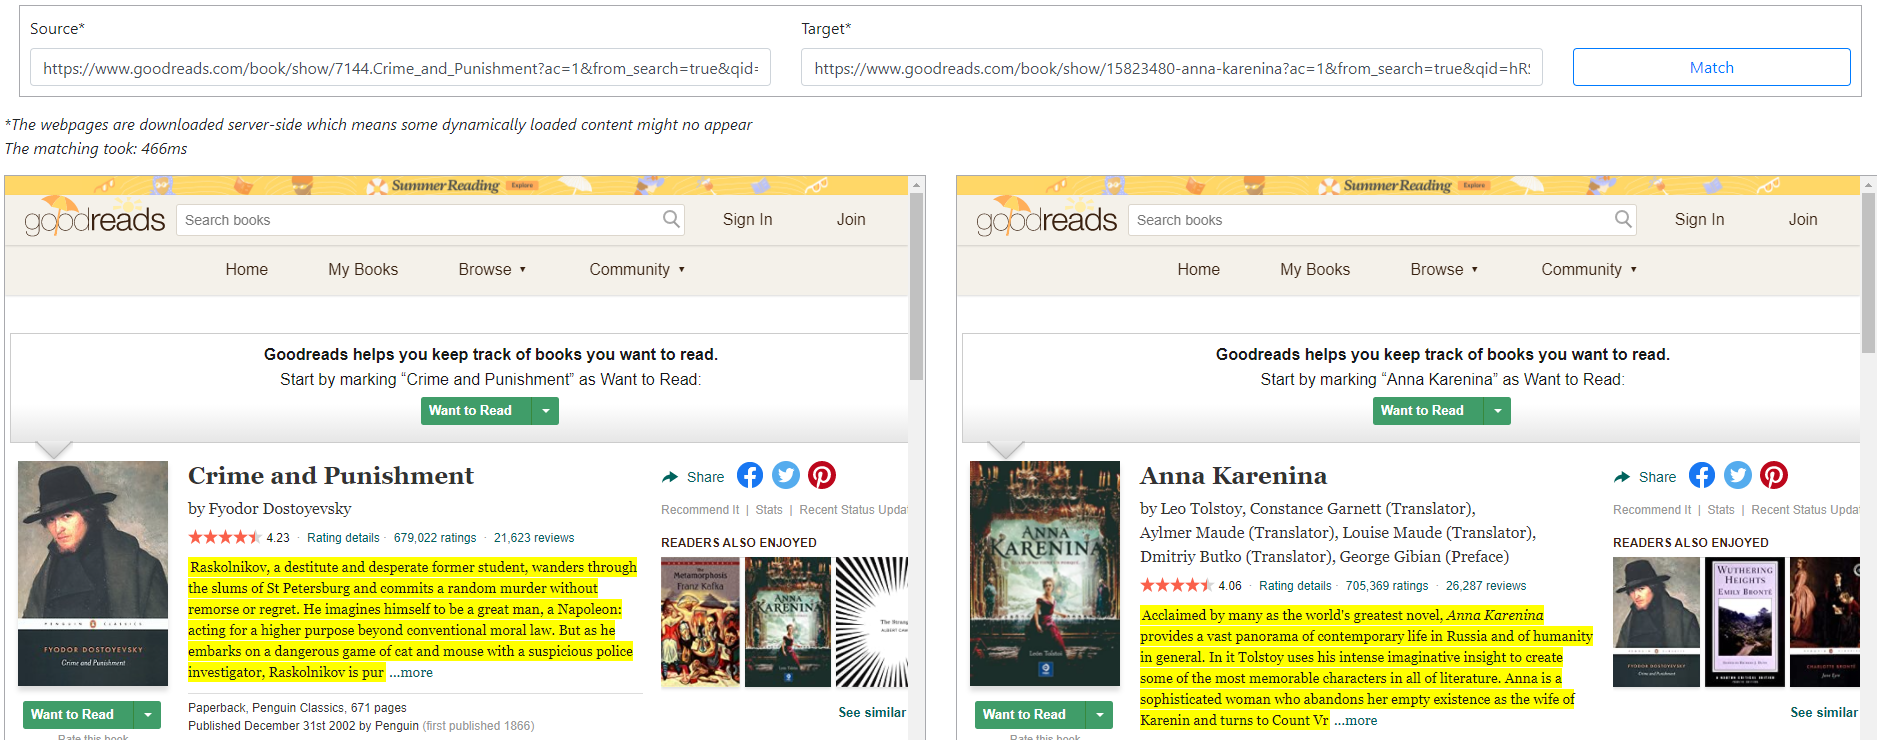
\includegraphics[width=\linewidth]{cerberus/explanations/demo_matching}
    \caption{The demo application developed to test \erratum on real use-cases before starting integration. In this example, the description of a book is hovered on the left-side webpage, which automatically highlights the matched element on the right-side webpage.}
    \label{fig:demo_app}
\end{figure*}

The application also allows users to input HTML files, which allowed to test the matching algorithm on several alternative versions of pages.
This demonstration step constituted a crucial step of the integration process by convincing the \cerberus community of the benefit brought by \erratum with regards to existing support for web locators.
Practitioners quickly understood that the algorithms of \erratum~\cite{brisset2021erratum,brisset2020sftm} could automate most of the situations they were facing during the web testing campaigns.
Furthermore, the fact that \erratum preserved the separation of concerns between the web application and the testing campaign emerged as another convincing argument in favour of \erratum.
Once validated, we moved forward by studying the integration strategies to implement this research results into the open-source platform.

\subsection{Integration Strategies in \cerberus}
Two main strategies were investigated:
\begin{inparaenum}[\em (i)]
\item use \erratum to automatically repair broken locators by fixing automated tests, or
\item use \erratum directly in the \cerberus testing environment, as an alternative way to locate elements.
\end{inparaenum}

The first approach reflects the case study considered in the original \erratum article~\cite{brisset2021erratum}.
The main benefit of this approach is that it can be seamless for the tester: whenever a locator breaks, it is automatically repaired without requiring any action from the tester.
However, integrating such a solution implies some significant changes in the \cerberus architecture.
Indeed, given a locator $l = loc_{e,D}$ that identifies en element $e \in D$, if $l$ breaks on $D'$, then \erratum requires to recover the original page $D$ on which the locator was initially working.
Since the history of pages is not recorded by \cerberus, the repair approach would require some major structural changes to keep track of web application histories.

As a first iteration, we therefore chose the second strategy.
Instead of using \erratum as a locator repair method, we consider its extension as a robust locator method to replace standard locators, like \textit{CSS} or \textit{XPath}, as described in Section~\ref{sec:erratum}.
Interestingly, the existing support for multiple classes of web locators in \cerberus offers a more straightforward hook to integrate \erratum.

\subsection{The \erratum Robust Locators}
To leverage the integration of \erratum in \cerberus, we therefore packaged \erratum as a robust locator.
The key property that differentiates \erratum from other web locators is that \erratum requires the original DOM $D$ on which the element was successfully located.
To build a robust locator with \erratum, we embedded the whole DOM $D$ in the locator---\emph{i.e.}, the \erratum locator of an element $e \in D$ is the pair $(XPath(e), D)$, where $XPath(e)$ is the absolute XPath of $e \in D$.
Figure~\ref{fig:erratum_as_locator} depicts how we extended \erratum to implement to robust locator support in \cerberus:
\begin{compactenum}
    \item from the original page $D$, the tester selects the element to locate $e$,
    \item so far, with XPath:
    \begin{compactenum}
        \item the tester specifies the web locator as an XPath query that she thinks to be robust to select $e \in D$,
        \item during the test execution, the XPath query is executed on the new DOM $D'$. If the locator is not broken, the query evaluation returns $e'$, but if the XPath query fails, then the test scenario is likely considered as broken,
    \end{compactenum}
    \item while, with \erratum{}:
    \begin{compactenum}
        \item the web locator is automatically generated, as a pair $(XPath(e), D)$, where $XPath(e)$ is the absolute XPath of $e$ and $D$ is the full DOM,
        \item during the test execution, \erratum{} first matches all the elements of $D'$ with $D$, and then the resulting matching is used to relocate the matched element $e \in D$ into $e' \in D'$.
    \end{compactenum}
\end{compactenum}

\begin{figure*}[htbp]
    \centering
    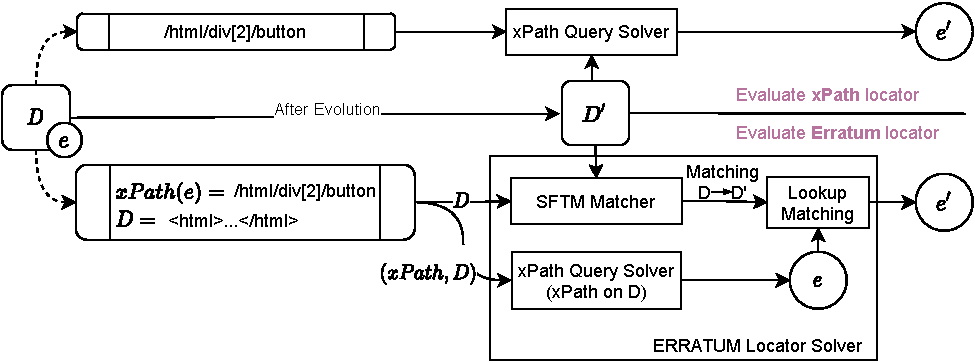
\includegraphics[width=.7\linewidth]{cerberus/explanations/erratum_as_locator}
    \caption{Describing how \erratum is integrated as a robust locator in \cerberus. Both locator types originally locate an element $e \in D$. The figure illustrates the ways \cerberus evaluates XPath or \erratum locators on a new DOM $D'$.}
    \label{fig:erratum_as_locator}
\end{figure*}

% Addressing the integration of \erratum through the robust locator problem rather than locator repair is a subtle pivot that eases the implementation, as it allows \erratum to be included in a similar way to already existing locator methods, like \textit{XPath} or \textit{CSS}.

To allow this integration within \cerberus, we rewrote the generic matching algorithm of \erratum, namely SFTM~\cite{brisset2020sftm}, in a language that can compile to JVM.
The code of the resulting library is open-source\footnote{\url{https://github.com/lssol/sftm\_tree\_matching}} and the library is published in Maven central.\footnote{\url{https://mvnrepository.com/artifact/io.github.amaris/sftm-tree-matching}}
Then, the integration of the \erratum library in the \cerberus platform represents only 127 lines of Java code.\footnote{\url{https://github.com/cerberustesting/cerberus-source/commit/0a70d4cc0d70a797901652fd2b97d501bb7fa511}}

\subsection{Usage}
The usage of the new \erratum locator on Cerberus is very similar to that of other locators.
Given an element $e$ that the tester wants to select on the page $p$, she has to:
\begin{compactenum}
\item select the \erratum locator type on the test case select box (see figure~\ref{fig:cerberus}), and then
\item copy-paste the absolute XPath of $e$ and the whole HTML of $p$ in the input form.
\end{compactenum}
To ease this process, we developed a browser extension allowing to simply click on the targeted element $e$ to copy the required data in the clipboard before pasting it into the input form.

In addition to providing more robust locators, writing test scenario using \erratum along with its extension represents a significant time gain: instead of manually crafting a locator that the tester judges to be robust enough, she simply needs to click on the targeted element. 
It allows the tester to completely ignore the details of how a certain element should be located and instead focus on building the most relevant test scenarios.

\section{Industrial Impact}\label{sec:impact}
Every year, the \laredoute{} web testing team estimated that the locator breakage entailing the failure of their test campaigns induced more than 11\,K\texteuro{} worth of load to their teams.
For industrial projects that evolve quickly, some testing campaigns were even cancelled because of the cost to continuously repair the broken test scripts.
In addition to that, repairing broken locators was considered as a tedious low-value task, which may be harmful to the moral of testers. 
We collected the feedbacks of 2 testers from this team, mainly asking about the biggest pain points faced by the testing team and how a solution like \erratum could help. 
According to the most experience tester we interviewed, most challenges faced by the test team stem from the separation between the development team and the testing team.
The development team is encouraged to push features fast (pressure on quantity), while the testing team's role is to monitor the quality of the released application.
The problem is all the more aggravated by the fragility of the developed test cases: when a new version is released, it takes several days to fix all tests which means that when the tests are ready, the developers are already working on different features.
Hence, using a tool like \erratum helps tightening the feedback loop between the testing team and the development team, thus allowing more intricate collaboration and less friction.

\laredoute{} unfortunately does not conserve a history of failed tests (along with the web page versions), which makes it hard to quantitatively measure the exact percentage of successful relocation of \erratum on their industrial cases.
We collaborated with 5 testing experts working on different campaigns to evaluate \erratum. 
The purpose of this evaluation was mainly to assess if \erratum could be used systematically in place of manually written \textsc{XPath} to locate elements on new tests cases, which would significantly fasten their development and maintenance.
We tried to design evaluation strategies that would not require too much time from the testing experts.
In particular, there were three stages of testing:
\begin{enumerate}
    \item Each tester tested 2 to 3 typical pages from their testing campaigns on the demo described earlier (see section~\ref{sec:demo});
    \item After \erratum was integrated to \cerberus, the \erratum locator type was tested on the same pages within the \cerberus framework;
    \item For two campaigns, each new test case written by the testers was duplicated for a period of one month: one version used an XPath locator and the other version, the \erratum locator.
\end{enumerate}

\begin{table}[]
\centering
\begin{tabular}{l|r|r|}
\cline{2-3}
                                                       & \bf Campaign A & \bf Campaign B \\ \hline
\multicolumn{1}{|l|}{\# Test cases}                        & 16         & 3          \\ \hline
\multicolumn{1}{|l|}{\# Releases}                          & 16         & 2          \\ \hline
\multicolumn{1}{|l|}{\# Locators / test (avg)}             & 18         & 22          \\ \hline
\multicolumn{1}{|l|}{\# Relocations}                       & 4,608       & 132         \\ \hline
\multicolumn{1}{|l|}{{[}XPath{]} \# Locator Failure} & 0          & 1          \\ \hline
\multicolumn{1}{|l|}{{[}\erratum{}{]} \# Locator Failures} & 0          & 0          \\ \hline
\end{tabular}
\caption{Results of the third testing phase that lasted one month.}
\label{table:results}
\end{table}

The evaluation of \erratum attempted to answer two questions:
\begin{enumerate}
\item Is \erratum a viable locator replacement of XPath?
\item Are \erratum locators more robust than manually written XPath locators?
\end{enumerate}

Table~\ref{table:results} presents the results of the third testing phase.
The campaign A applies to an application being completely rewritten, which explains the high frequency of releases.

During a month, there were $4,740$ locator relocations (\# tests $\times$ \# releases $\times$ average \# locators / test) over the two campaigns under study.
For \erratum, none of these relocations failed, while one failed for XPath.

The results thus tend to indicate that \erratum can be safely used as a replacement of manually written {\sc XPaths}.
As for whether \erratum provides more robust locators than manually written XPath, there is still not enough data to conclude. 

Following the evaluation, \laredoute{} now adopted \erratum as the preferred locator method, along with \texttt{data-cerberus} attributes, and have not yet reported any relocation failure at the time of writing this paper.
Beyond the collaboration with \laredoute, we believe that these promising results will benefit to the wider \cerberus community.

\section{Perspectives}\label{sec:perspectives}
\paragraph{Visual integration}
considering the above \erratum web extension, the tester no longer needs to analyze the HTML source code and manually assemble a robust locator.
It means that, theoretically, \cerberus could integrate a fully visual locator selection approach where
\begin{inparaenum}[\em (i)]
    \item the tester fills in the web application URL,
    \item the page opens in an iframe,
    \item the tester selects the target element,
    \item the \erratum locator is automatically generated.
\end{inparaenum}
This process was originally considered, however, it would not be usable in more complex situations where some pages are not directly accessible from a given URL (\emph{e.g.}, a page that requires to login first).

\paragraph{Mobile testing}
the web testing teams in the \laredoute{} company also use \cerberus to automate tests from mobile devices.
Web pages are described using HTML and Android views are written in XML.
While HTML and XML are very similar and our tree matching library theoretically allows \erratum to match any kind of tree (and not only HTML trees), some technical adjustments still need to be completed to include XML trees in \cerberus.
Furthermore, the robustness of \erratum's locators to typical Android XML view mutations still need to be assessed, as they may differ from typical HTML mutations.

\section{Conclusion}\label{sec:conclusion}
Web locators remain a fragile keystone of automated test suites executed by modern test platforms.
Whenever a locator fails to locate a web element in a test suite, it directly impacts the whole test campaign and impose some additional maintenance tasks to the web testing team.

In this paper, we described how we extended and successfully integrated the locator repair solution \erratum into \cerberus, a widely used open source test-automation solution.
In particular, we reported on the development of a robust locator based on \erratum that eases the pain of web testers, by saving time and reducing the cost of test campaigns.
